% --------------------------------------------------------------------------- %
% --------------------------------------------------------------------------- %
\chapter{Introduction}
\label{ch:intro}
% --------------------------------------------------------------------------- %
% --------------------------------------------------------------------------- %

\section{Particle Physics}
The goal of particle physics is to answer the question, what is matter composed of and how do different types of matter interact?
Using the theory of the Standard Model, physicists have been very successful in answering this question for a variety of interactions.
The standard model isn't able to explain everything however, for example the observation of dark matter and dark energy in the universe are not explained by the standard model.
There are many theories that have been proposed which can explain these phenomena.
Supersymmetry is an extension of the standard model which proposes an explanation for dark matter.

\section{The Standard Model}
The standard model of particle physics is one of the most successful theories of all time.
The theory is used to describe the composition of fundamental constituents of matter and how they interact.
According to the standard model, matter is made up of two types of elementary particles, fermions and bosons.
Fermions are particles that have half-integer spin, and bosons have integer spin.
Matter is made up of fermions, and matter interacts when fermions exchange bosons.
There are two types of fermions, quarks and leptons, and each of these consist of 6 flavors.
Quarks are divided into two categories, up-like (charge = 2/3e) and down-like (charge = -1/3e).
The up-like quarks are named up, charm and top and the down-like quarks are named down, strange, and bottom.
Leptons are also divided into two categories, charged (charge = 1e) and neutral.
Each charged lepton has neutral partner called a neutrino, and the lepton flavors are named electron, muon, tau.
In addition, every particle in the standard model has an anti-particle partner.
This anti-particle is exactly the same except the sign of all charges (electric and color) are the opposite value of the original charge.

There are 4 known forces in the universe, the gravitational force, the weak force, the electromagnetic force, and the strong force.
With the exception of gravity, these forces are explained by the standard model as the exchange of bosons between fermions.
According to the standard model, the weak force is governed by the Z0 and $\mathrm{W^{+}~and~W^{-}}$~bosons,
the electromagnetic force is governed by the photon, and the strong force is governed by the gluon.
In 2012, it was announced that a new particle was discovered at the LHC by the CMS~\cite{discovery} and ATLAS~\cite{higgsatlas} experiments.
This particle has properties consistent with that of a standard model Higgs boson.
The Higgs boson is responsible for the mass of the massive standard model particles.
A diagram of all the particles making up the standard model is shown in figure~\ref{fig:SM}.

\begin{figure}[!htb]
  \begin{center}
    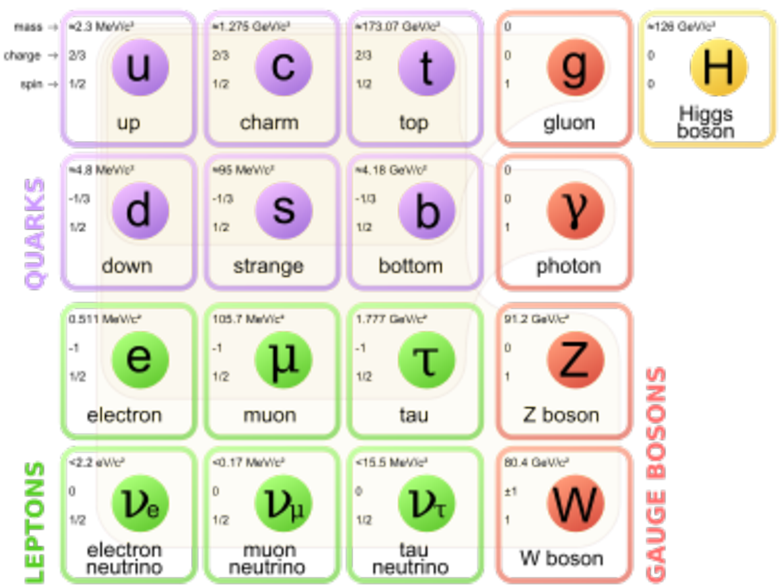
\includegraphics[width=0.8\textwidth]{intro/figs/Standard_Model_of_Elementary_Particles.pdf}
    \caption{
      \label{fig:SM}
      A diagram is shown with the particles making up the Standard Model along with the attributes of each particle.
    }
  \end{center}
\end{figure}

R-parity is a concept that is defined in equation~\ref{eqn:rparity} where B = baryon number, L = lepton number, and s = spin. 
Baryon number is defined in equation~\ref{eqn:baryonnumber},
where $\mathrm{N_{q}}$ and $\mathrm{N_{\bar{q}}}$ are the number of quarks and anti-quarks respectively.
Lepton number is defined in equation~\ref{eqn:leptonnumber},
where $\mathrm{N_{L}}$ and $\mathrm{N_{\bar{L}}}$ are the number of leptons and anti-leptons respectively.
All particles in the standard model have $\mathrm{P_{R}} = 1$.

\begin{equation}
\label{eqn:rparity}
\mathrm{P_{R} = (-1)^{3(B-L)+2s}}
\end{equation}

\begin{equation}
\label{eqn:baryonnumber}
\mathrm{B = \frac{1}{3}(N_{q}-N_{\bar{q}})}
\end{equation}

\begin{equation}
\label{eqn:leptonnumber}
\mathrm{L = N_{L}-N_{\bar{L}}}
\end{equation}

\subsection{Problems with The Standard Model}
The standard model is able to explain many things, but it is not complete.
One example of where it fails is in explaining the existence of ``dark matter''.
Dark matter is a form of matter that does not interact electromagnetically and has been observed by astrophysicists~\cite{darkmatter}.
Dark matter has been measured to be \textasciitilde{}5 times more abundant than visible matter in the universe.
The hierarchy problem is another question that is not explained by the standard model,
which essentially asks why is the weak force more than 1000 times stronger than gravity?
One of the main goals of particle physics is to understand and provide explanations for these problems,
and one way this can be done is within the context of supersymmetry (SUSY).

\section{Supersymmetry (SUSY)}
SUSY~\cite{SUSYPrimer} is an idea which postulates that for every particle in the standard model,
there exists a supersymmetric partner which has the property that the partners to bosons is fermionic, and the partners to fermions are bosonic.
These particles are named sparticles, and for fermions, an s, short for scalar, is added to the beginning of the standard model particle name to represent the SUSY particle.
A diagram of this is shown in figure~\ref{fig:SM_SUSY}.
For example, a supersymmetric electron is known as a selectron, and a supersymmetric quark is known as a squark.
For gauge bosons, the end of the name is changed to contain ``ino''.
For example, the supersymmetric partner to the W boson is known as the Wino and a supersymmetric gluon is known as a gluino.
R-parity is an important concept within SUSY, and all SUSY particles have $\mathrm{R_{P}} = -1$.
This means that if R-parity is conserved, the lightest supersymmetric particle (LSP) in a decay is stable.
The LSP then makes a good candidate for dark matter.
Using SUSY as a framework, one can create many models that can answer both the hierarchy problem as well as explain the existence of dark matter.
This thesis focuses more on a search for new physics within SUSY that can be used as an explanation for dark matter.

\begin{figure}[!htb]
  \begin{center}
    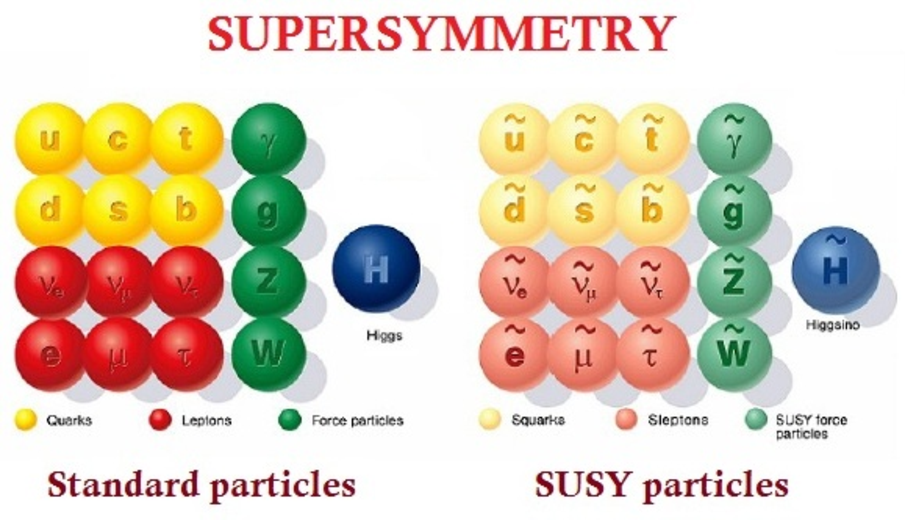
\includegraphics[width=0.8\textwidth]{intro/figs/Susy-particles.pdf}
    \caption{
      \label{fig:SM_SUSY}
      A diagram is shown with the particles making up the Standard Model on the left, and their SUSY counterparts on the right.
    }
  \end{center}
\end{figure}

%% \subsection{Gauge-Mediated Supersymmetry Breaking (GMSB)}
%% Gauge-Mediated Supersymmetry Breaking (GMSB) is a mechanism that allows supersymmetry to be broken.
%% This mechanism postulates the existence of a particle that can be used to explain gravity as well as dark matter, the gravitino ($\mathrm{\tilde{G}}$).
%% Within SUSY, the hierarchy problem can be solved with one loop corrections coming from heavy stop quarks,
%% and another consequence of GMSB is the proposal that stop quarks must have a mass greater than 2 TeV if the Higgs mass is 125 GeV.
%% The current upper limits on the mass of the stop squarks based on observations made by the CMS detector are around 800 GeV~\cite{stop2015}, as seen in figure~\ref{fig:T2tt_limits}.

%% \begin{figure}[!htb]
%%   \begin{center}
%%     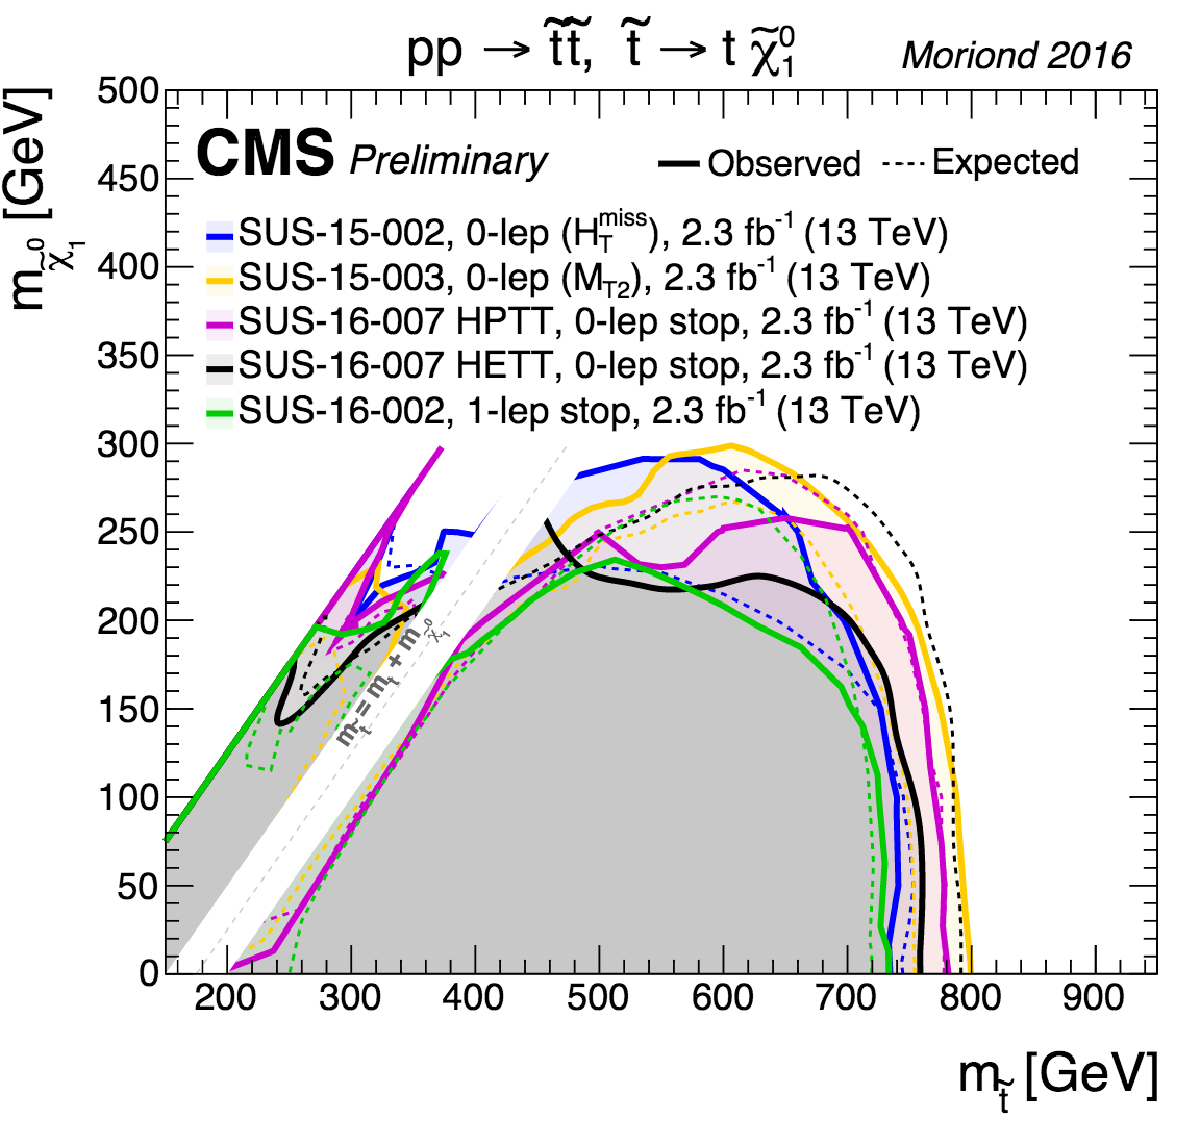
\includegraphics[width=0.8\textwidth]{intro/figs/T2tt_moriond2016.pdf}
%%     \caption{
%%       \label{fig:T2tt_limits}
%%       Exclusion limit on the SUSY final states where two stop squarks are pair-produced are shown,
%%       where the region in gray has been excluded by data taken by the CMS experiment.
%%     }
%%   \end{center}
%% \end{figure}

\section{Searches for SUSY in final states with a Z boson}
\label{sec:signalmodel}
Many models can exist within the context of SUSY, leading to a nearly endless variety of final states.
There are many parameters within SUSY that can be tuned to allow for the existence of different final states, for example the mass of the SUSY particles.
A set of simplified models can be described to get a sense of what possible final states can be probed using the CMS detector at the LHC.
These models are named SMS models, where SMS stands for Simplified Model Space~\cite{sms}.
One of these models, shown in figure~\ref{fig:SMS_T5ZZgmsb}, is a model with a final state containing two Z bosons,
four quarks and two invisible SUSY particles where the invisible particles in this model are the gravitino.
This thesis focuses on a search done using data taken by the CMS detector at the LHC colliding protons with a center of mass energy of $\mathrm{\sqrt{s}=13 TeV}$.
The next chapter will explain in detail how particles are measured using the CMS detector.

\begin{figure}[!htb]
  \begin{center}
    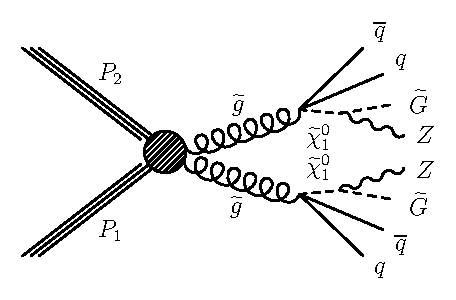
\includegraphics[width=0.8\textwidth]{intro/figs/Feynman_graph_T5ZZgmsb.pdf}
    \caption{
      \label{fig:SMS_T5ZZgmsb}
      A diagram showing a SUSY process where two protons collide and the result is pair-production of two gluinos,
      where each decays to a pair of quarks and a neutralino which subsequently decays to a Z boson and gravitino.
    }
  \end{center}
\end{figure}

This is to acknowledge all the other members of the CMS experiment who made it possible to produce
the figures and tables appearing in this chapter.
